\question (北京航空航天大学,2004年)若图的邻接矩阵主对角线上的元素皆为0,其余元素全为1,则可以断定该图一定(
)
\par\twoch{是无向图}{是有向图}{\textcolor{red}{是完全图}}{不是带权图}
\begin{solution}任意两个结点都有边直接相连,必然是完全图。但不能确定是否是无向图。因此A、B都不可,也无法确定是否是带权图,因为权值可以为1。
\end{solution}
\question (武汉大学,2000年)用相邻矩阵A表示图,判定任意两个顶点vi和vj之间是否有长度为m的路径相连,则只要检查(
)的第i行第j列是否为零即可
\par\twoch{mA}{A}{\textcolor{red}{}}{}
\begin{solution}这类题目可先用特殊法,如m=1时,马上可以排除D。 如m=2时,排除A和B。
因此本题选C。
下面拿m=2的情况,进行证明。若vi、vj之间存在长度为2的路径,设此路径经过顶点vk,则存在边和。因此Aik和Akj都不为0,因此{[}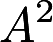
\includegraphics[width=0.18750in,height=0.15625in]
{texmath/99dc305Cdpi7B3507DA5E2}{]}i,j=Aik*Akj≠0。因此C是正确答案。
\end{solution}
\question (北京交通大学,2004年)n个顶点、e条边的有向图的邻接矩阵中非零元素有(
)个
\par\twoch{n}{2e}{\textcolor{red}{e}}{n+e}
\begin{solution}有向图的非零个数等于其边数。
\end{solution}
\question (华中科技大学,2006年)n个顶点的无向图的邻接表最多有( )个表结点
\par\fourch{\textcolor{red}{}}{n(n-1)}{n(n+1)}{n(n-1)/2}
\begin{solution}每个顶点后面最多跟n-1个边表节点。加上顶点本身,每个单链表最多有n个表结点,又最多有n个这样的单链表,那么最多就有n*n=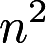
\includegraphics[width=0.16667in,height=0.15625in]{texmath/071fa15Cdpi7B3507Dn5E2}个表结点。
\end{solution}
\question (华南理工大学,2006年)下列对邻接表的叙述中,( )是正确的
\par\fourch{无向图的邻接表中,第i个顶点的度为第i个链表中结点数的2倍}{邻接表比邻接矩阵的操作更简便}{邻接矩阵比邻接表的操作更简便}{\textcolor{red}{求有向图结点的度,必须遍历整个邻接表}}
\begin{solution}A中不是2倍是1倍。
B、C中,错误的原因跟``线性表中链表比顺序表操作更简便''一样。只有在设定的前提下,才有哪个更简便,更好的说法。
\end{solution}
\question (中南大学,2004年)在有向图的邻接表存储表示中,顶点V在链表结点中出现的次数是(
)
\par\twoch{\textcolor{red}{顶点V的入度}}{顶点V的出度}{顶点V的度}{依附于顶点V的边的数目}
\begin{solution}邻接表记录各个顶点到各个点的边情况,所以出现的次数即是到达该顶点的数目,也就是入度。比如链表adjlist{[}0{]},记录的就是0结点所到达的各个点的边。
\end{solution}
\question (中国科学院,2007年)若邻接表中有奇数个表结点,则一定是( )
\par\twoch{图中有奇数个结点}{图中有偶数个结点}{图为无向图}{\textcolor{red}{图为有向图}}
\begin{solution}无向图的邻接表的表结点个数为边数的两倍,即一定为偶数,因此出现奇数个表结点的一定是有向图,跟顶点(结点)数量无关。
\end{solution}
\question 下列关于图的叙述,正确的是( )。 Ⅰ.回路是简单路径
Ⅱ.存储稀疏图,用邻接矩阵比邻接表更省空间
Ⅲ.若有向图中存在拓扑序列,则该图不存在回路
\par\twoch{仅Ⅱ}{仅Ⅰ、Ⅱ}{\textcolor{red}{仅Ⅲ}}{仅Ⅰ、Ⅲ}
\begin{solution}若路径中除了开始点和结束点可以相同以外,其余顶点均不相同,则称这条路径为简单路径。若一条路径中第一个顶点和最后一个顶点相同,则这条路径是一条回路(回路中可能存在既不是起点也不是终点的相同点),故Ⅰ错误。后话,要是两者是充要条件,也就不必要两个名词了。
邻接矩阵无论图是稀疏还是稠密,都取的是最大的存储空间,因此用邻接表比邻接矩阵更省空间,故Ⅱ错误。
用拓扑排序的方法可以判断图中是否存在回路,如果对一个图可以完成拓扑排序,则此图不存在回路,故Ⅲ正确。
【总结】
本题考查了图的多个知识点,但本题目出的不是很好,属于3个比较简单的判断题的生硬拼凑,不能算是好的``综合''题。但做题的同学需要掌握多个基础知识点才可正确解答。
\end{solution}
\question 设图的邻接矩阵A如下图所示。各顶点的度依次是( ~)。~

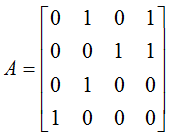
\includegraphics[width=1.77083in,height=1.43750in]{computerassets/596518D94738A905011156D7D79F7DEE.png}
\par\fourch{1,2,1,2}{2,2,1,1}{\textcolor{red}{3,4,2,3}}{4,4,2,2}
\begin{solution}各顶点的度包括了入度和出度,因此是矩阵中此结点对应的横行和纵列非零元素之和,所以可得各顶点的度分别为3,4,2,3。
\end{solution}
\question (中科院,2004年)下面关于图的存储的叙述中正确的是( )
\par\fourch{\textcolor{red}{用邻接矩阵法存储图,占用的存储空间大小只与图中顶点数有关,而与边数无关}}{用邻接矩阵法存储图,占用的存储空间大小只与图中边数有关,而与顶点数数无关}{用邻接表法存储图,占用的存储空间大小只与图中顶点数有关,而与边数无关}{用邻接表法存储图,占用的存储空间大小只与图中边数有关,而与顶点数无关}
\begin{solution}用邻接矩阵法存储图的时候,矩阵的大小为n*n,其中n为图的顶点数,所以占用的存储空间只与图中顶点数有关,而与边数无关。用邻接表法存储图,有边表和顶点表,所以占用的存储空间与图中的顶点数和边数都有关
\end{solution}
